\chapter[Partial Differential Equations]{Partial Differential Equations}

\section[Lecture 1 (02-03) -- {What are the PDEs?}]{Lecture 1 (02-03)Initial and Boundary Conditions}

\subsection{What are the PDEs?}
\begin{align}
    \label{eq1} \pdv{u}{t}=\pdv[2]{u}{x}+\pdv[2]{u}{y}-u 
    \\ u=u(x,y,t)
\end{align}
\eqref{eq1} is a second order PDE
 

\subsection{Classical solutions}
To simplify, we consider here equations of one unknown function $u$ of one or more variable
\\By a solution we mean a sufficiently smooth function $u$ that satisfies the PDE at every point of the domain of its definition($D$).
\\Sometimes, we will have to impose some boundary conditions on the domain $D$.
\\$C^n=\{u:D \rightarrow R:$ n-times continuous differentiable w.r.t all variables  \} $n$ is the order of the equation
\begin{example}{1}{}
    \begin{itemize}
        \item Heat equation: \[\pdv{u}{t}=\pdv[2]{u}{x}\]
        \[u=u(x,t)\]
        \[(t,x) \in D \subset R^2\]
        \[u(t,x), \pdv{u}{t}(t,x),\pdv{u}{x}(t,x),\pdv[2]{u}{x}(t,x),\pdv[2]{u}{t}(t,x)\]
        \[n=2\]
        \[\pdv{u}{x}{t}=\pdv{u}{t}{x} \in C^2\]
        \[u \in C^2(D)\]
        \item Some Solution:
        \[u(t,x)=t+\frac{x^2}{2},D=R^2\]
        \[u(t,x)=\frac{e^{-\frac{x^2}{4t}}}{2\sqrt{\pi t}},D=\{(t,x):t>0\}\]
        \[u(t,x)=e^{-t+ix}=e^{-t}cos(x)+ie^{-t}sin(x),D=R^2\]
    \end{itemize}
\end{example}
\subsection{Initial and Boundary Conditions}
What is Initial data?
\\$u(0,x)=u_0(x)$
\\
\\What are Boundary Conditions?
rigurous definition of Boundary
\begin{itemize}
    \item Dirichlet Boundary Condition: $u(t,x)|_{\partial{D}}=g(t,x)$
    \item Neumann Boundary Condition: When the normal derivative of $u$ is specified $\pdv{u}{n}$ where $n$ is the normal to the boundary $\partial(D)$
    \[\frac{\partial u}{\partial n}(t,x) = g(t,x)\]
    \item Mixed Boundary Condition: Combination of Dirichlet and Neumann
\end{itemize}
\subsection{Linear and Nonlinear waves}
\subsubsection{Stationary waves}
\begin{align}
    \label{eq2} \pdv{u}{t}&=0
    \\u&=u(t,x)
\end{align}
This is a first order linear homogeneuous PDE
\\Solution of the form $u=u(t)=c, \forall c \in R$
\\Let's integral \eqref{eq2} :
\[ 0=\int_{0}^{t}\frac{\partial u}{\partial t}(s,x)ds=u(t,x)-u(0,x)\]
\\Thus if an initial conditional
\[u(0,x)=f(x)\]
\[u(t,x)=f(x), \forall t,x\] 
Thus for any given $f \in C^1(R)$, we have a solution of \eqref{eq2} and this is a stationary wave
\\The domain of this solution is $R$ if $f$ is defined everywhere on $R$
\\Power of domain to change the solution:
\\Consider the ODE:
$$\dv{u}{t}=0, D=(-\infty,0)\cup(0,\infty) $$
\\The solution is:
\[
    u(t)=\begin{cases}
        c_1, t<0
        \\c_2, t>0
    \end{cases}
    \forall c_1,c_2 \in R
\]
\\similarly, for the PDE in example \eqref{eq2}:
$$
    u(t,x)=\begin{cases}
        0, x>0
        \\x^2, x\leq0,t>0
        \\-x^2, x\leq0,t<0
    \end{cases}
$$ 
it is a $ \mathbb{C}^1 $ solution of \eqref{eq2} on $ \mathbb{R}^2\backslash\{(0,x):x\leq0\} $, so it is not a function of x alone\\
Actually, it is not hard to check that if u is a clasical solution to \eqref{eq2}, defined on domain $ D\subset\mathbb{R}^2 $ whose intersection with any horizontal line $D_a=D\cap\{(t,a):t\in \mathbb{R}\},\forall a\in \mathbb{R}  $ is either empty or a connected interval, then $ u(t,x)=f(x) $ is only a function of x.
\begin{figure}[H]
    \centering
    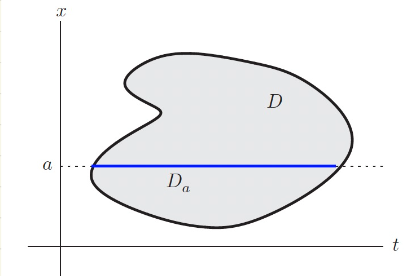
\includegraphics[height = 0.4\textwidth, width = 0.5\textwidth]{resource/1.png}
\end{figure}
\section[Lecture 2 (02-05) -- {Uniform Transport and Traveling waves}]{Lecture 1 (02-05)Transport and Traveling waves}
\subsection{uniform transport}
Let us consider the linear, homogeneuous first order PDE:
\begin{equation}
    \label{eq4} \pdv{u}{t}+c\pdv{u}{x}=0
\end{equation}
\begin{equation}
    \label{eq5} u=u(0,x)=f(x)
\end{equation}
$$
    x\in \mathbb{R},t_0=0,t-t_0=t,c\in \mathbb{R}
$$ 
\\\textbf{use change of variable:}  
$$
    \xi =x-ct
$$ 
$ \xi $ is called characteristic variable
\\let's look for a solution of \eqref{eq4} under the form $$ u(t,x)=v(t,\xi)=v(t,x-ct) $$ 
\textbf{use chain rule:}
$$
    \pdv{u}{t}=\pdv{v}{t}-c\pdv{v}{\xi}
$$ 
$$
    \pdv{u}{x}=\pdv{v}{\xi}
$$ 
Thus:
$$
    0=\pdv{u}{t}+c\pdv{u}{x}=\pdv{v}{t}-c\pdv{v}{\xi}+c\pdv{v}{\xi}= \pdv{v}{t}
$$ 
\textbf{Conclusion:}$$
    \pdv{v}{t}=0
$$ 
Solution is constant $ v(\xi) $
$$
u(t,x)=v(\xi)=v(x-ct)
$$  
\begin{proposition}{}{}
if u solves \eqref{eq4}, then u has the form $u(t,x)=v(x-ct)$ where v is a function of one variable that is $ \mathbb{C}^1 $-smooth.
\\Acutually, v is satisfying $$
    u(0,x)=v(x)=f(x)
$$ 
\end{proposition}
\textbf{Conclusion:}
$$\begin{cases}
    \pdv{u}{t}+c\pdv{u}{x}=0
    \\ 
    u=u(0,x)=f(x)
\end{cases}$$
The solution is $$ u(t,x)=f(x-ct) $$ 
\\$ f(x-ct) $ is a traveling wave solution moving at velocity $ c $:
\\if c>0, the wave moves to the right
\\if c<0, the wave moves to the left
\\if c=0, the wave is stationary 
\begin{example}{}{}
$$\begin{cases}
    \pdv{u}{t}+2\pdv{u}{x}=0
    \\ 
    u=u(0,x)=\frac{1}{1+x^2}
\end{cases}$$
The solution is $$ u(t,x)=\frac{1}{1+(x-2t)^2} $$
The lines $ x=ct+k $ are called the characteristic lines for the equation \eqref{eq4}
\\on the characteristic lines, the solution is always constant
\\on geometric interpretation, $u(t,x)=f(x-ct)=f(k)$
\end{example}
Consider the equation:
\begin{equation}
    \label{eq6} \pdv{u}{t}+c\pdv{u}{x}+au=0
\end{equation}
where a and c are given numbers.
\\\textbf{Use change of variable:}
$$
    u(t,x)=v(t,\xi)=v(t,x-ct)
$$ we will get by the same computation
$$
    \pdv{v}{t}+av=0
$$ 
\\The solution will be$$
    v(\xi)=e^{-at}f(\xi)
$$ 
$$
    u(t,x)=v(t,\xi)=v(x-ct)=e^{-at}f(x-ct)
$$ 
\\So,
$$
    \begin{cases}u(t,x)=e^{-at}f(x-ct)\\u(0,x)=f(x)\end{cases}
$$ 
\subsection{Nonuniform transport}
\begin{equation}
    \label{eq7} \pdv{u}{t}+c(x)\pdv{u}{x}=0
\end{equation}
\\In the uniform case(c constant), characteristic line is x=ct+k  (the solution of ODE below)
$$
    \dv{x}{t}=c
$$ 
\\In the general non-uniform case, we can still define characteristic curves
$$
    \frac{d}{dt}x(t)=c(x(t))
$$ 
\\Let's show that the solutions of \eqref{eq7} are constants along the characteristic curves (t,x(t))
\\We need to check that $ u(t,x(t))=h(t) $ is constant of t 
\\compute the derivative of $ h(t)$ 
\begin{align*}
    \frac{d}{dt}h(t) &= \frac{d}{dt}u(t,x(t)) = \pdv{u}{t}(t,x(t))+\pdv{u}{x}(t,x(t))\cdot\dv{x}{t} \\
    &= \pdv{u}{t}(t,x(t))+c(x(t)) \cdot \pdv{u}{x}(t,x(t)) = 0
\end{align*}
h(t) and thus u(t,x(t)) is constant along the characteristic curves
\begin{definition}{}{}
The graph of a solution of the ODE $$\frac{d}{dt}x(t)=c(x(t))$$ is called a characteristic curve for the transport equation \eqref{eq7} with speed c(x)
\end{definition}
Thus at each point (t,x) the slope of the characteristic curve is c(x) (the wave speed)
\\Thus, we proved:
\begin{proposition}{}{}
The solutions to the linear transport equation \eqref{eq7} are constant along the characteristic curves
\end{proposition}
In the particular case c(x)=c, the characteristic curves are straight lines of slope c
\\Moreover,
\\ \eqref{eq7} is an autonomous first order ODE which can be "solved" using the method of separation of variables
\\Assume that c(x)$ \neq $0 
\begin{align*}
    \frac{dx(t)}{dt}&=c(x(t))
\\\frac{dx}{c(X)}&=dt \rightarrow
\\ \beta (x)&=\int\frac{dx}{c(x)}=t+k
\end{align*}
\\Thus characteristic curves satisfies the implicit equatioin$$\beta(x)=t+k$$
\\We can find x from the equality using $ \beta^{-1} $(the inverse of $ \beta $) 
\begin{align*}
    \beta(x)&=t+k
    \\ \beta^{-1}\beta(y)&=y
    \\x(t)&=\beta^{-1}(t+k)
\end{align*}
\begin{remark}{}{}
How to determine where $c(x_0)=0$?
\\Solve this ODE$$
    \begin{cases}
        \frac{dx}{dt}=c(x)
        \\x(t_0)=x_0
    \end{cases}
$$ 
and $ x(t)=x_0 $ wil be the characteristic curve going through ($t_0,x_0$) 
\end{remark}
From the proposition, we know that $ u(t,x(t)) $=constant
\begin{align*}
    u(t,x(t))&=v(k)
    \\&=v(\beta(x(t))-t)
\end{align*} 
\\where k is the constant determining the characteristic curve (t,x(t))
\begin{align*}
    u(t,x)=v(\xi)
    \\ \text{where    } \xi=\beta(x)-t
\end{align*}
\\which we will call characteristic variable
\begin{equation}
    \label{eq8} u(t,x)=v(\beta(x)-t)
\end{equation}
\\This formula way fail at points where c vanishes
\begin{align*}
    t&=0
    \\u(0,x)=f(x)&=v(\beta(x)-0)
    \\f(x)&=v(\beta(x))
    \\v(\xi)&=f(\beta^{-1}(\xi))
    \\&=f\cdot \beta^{-1}(\xi)
    \\u(t,x)&=f\cdot\beta^{-1}(\beta(x)-t)
\end{align*}
\\This is the formula for the solution of  \eqref{eq7} in the general case
\\which is:$$\begin{cases}
\pdv{u}{t}+c(x)\pdv{u}{x}=0
\\u(0,x)=f(x)
\end{cases}
$$ 
\begin{example}{}{}
Let us apply the method of characteristics to solve the nonuniform transport equation:
$$
    \pdv{u}{t}+\frac{1}{x^2+1}\pdv{u}{x}=0
$$ 
The characteristic curves are the graphs of the solutions of the ODE:
$$
    \dv{x}{t}=\frac{1}{x^2+1}
$$ 
\begin{align*}
    \Rightarrow \beta(x)&=\int(x^2+1)dx\\
    &=\frac{x^3}{3}+x\\
    &=t+k
\end{align*}
It is not particularly helpful to find x(t) form this equation.\\
characteristic variable $ \xi $ is given by $ \xi=\frac{x^3}{3}+x-t $ and the general solution is of the form
$$
    u=v(\frac{x^3}{3}+x-t)
$$  
where v is any $ \mathbb{C}^1 $ function.\\
\begin{figure}[H]
    \centering
    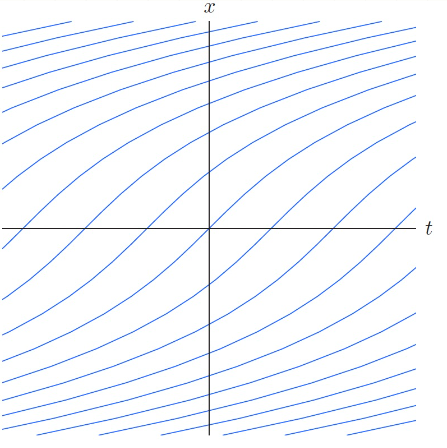
\includegraphics[height = 0.4\textwidth, width = 0.5\textwidth]{resource/2.png}
    \caption{Characteristic curves for $u_t+(x^2+1)^{-1}u_x=0$}
	\label{img:chcurve}
\end{figure}
In the case of the initial condition:
$$
    u(0,x)=\frac{1}{1+{(x+3)}^2}
$$  
The solution looks as follows:
\begin{figure}[H]
    \centering
    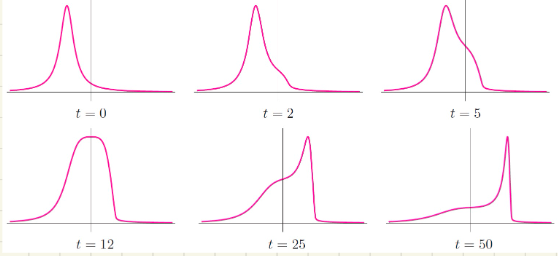
\includegraphics[height = 0.4\textwidth, width = 0.5\textwidth]{resource/3.png}
\end{figure}
\end{example}
\section{Lecture 3 (02-10)-Nonlinear transport and shocks}
Nonlinear transport equation:
\begin{equation}
   \label{eq9} \pdv{u}{t}+u\pdv{u}{x}=0
\end{equation}
characteristic equation:
\begin{equation}
    \label{eq10}\dv{x(t)}{t}=u(t,x(t)),\text{ x(t) is the characteristic curve} 
\end{equation}
Let's show that u the solution of \eqref{eq9} is constant along the characteristic curves x(t)
\\we need to check that $ h(t)=u(t,x(t)) $ is constant of t
\begin{align*}{}{}
\frac{d}{dt}h(t)&=\pdv{u}{t}(t,x(t))+\pdv{u}{x}(t,x(t))\cdot\dv{x}{t}\\
&=\pdv{u}{t}(t,x(t))+\pdv{u}{x}\cdot u(t,x(t))\\
&=0 (\text{ by }\eqref{eq9})
\end{align*}
As u is constant along the characteristic curves, it must be of the form function of characteristic variable:
\begin{align*}{}{}
    \xi=x-ut
\end{align*}
\begin{equation}
    \label{eq11} u(t,x)=f(x-tu(t,x))
\end{equation}
\begin{example}[]{}
 Suppose the initial data is:
 $$
    f(\xi)=\alpha \xi+\beta
 $$ 
 Then \eqref{eq11} becomes:
 \begin{align*}{}{}
 u=\alpha(x-tu)+\beta 
 \end{align*} 
 \begin{equation}
        \label{eq12} u(t,x)=\frac{\alpha x+\beta}{1+\alpha t}
 \end{equation} 
 As far as $ 1+dt\neq 0 $, the graoh of the solution is line 
 \\If $ \alpha>0 $ ,\begin{align*}{}{}
 u(t,x)\rightarrow 0\\
 t\rightarrow +\infty
 \end{align*} 
If $ \alpha<0 $ , then the solution blows up as $ t\rightarrow -\frac{1}{\alpha} $
since $ \dot{x}=u(t,x(t)) $
\\As u(t,x(t))is a constant ,
\begin{align*}{}{}
u(t,x(t))&=u(0,x(0))\\
&=u(0,y)\\
&=f(y)
\end{align*}
Our characteristic ODE is:
\begin{align*}{}{}
\dot{x}&=f(x)\\
\Rightarrow x(t)&=tf(y)+y\\
\Rightarrow u(t,x(t))&=u(t,tf(y)+y)\\
&=u(0,y)\\
&=f(y), \forall t\\
u(t,tf(y)+y)&=f(y) \forall t, y\\
u(t,x)&=f(y)\\
x&=tf(y)+y
\end{align*}
I find $ y\in \mathbb{R} $
Suppose let $ f(y)=y $
\begin{align*}{}{}
x=ty+y,y=\frac{x}{t+1}\\
\Rightarrow u(t,x)=f(y)=y=\frac{x}{t+1}\\
\Rightarrow u(t,x)=\frac{x}{t+1}
\end{align*}  
which agrees with \eqref{eq12} for $ \alpha=1,\beta=0 $\\
There is a problem with this construction that becomes clear when considering the following example:
$$
    u(0,x)=f(x)=\frac{1}{2}\pi-tan^{-1}(x)
$$ 
\begin{figure}[H]
	\centering
	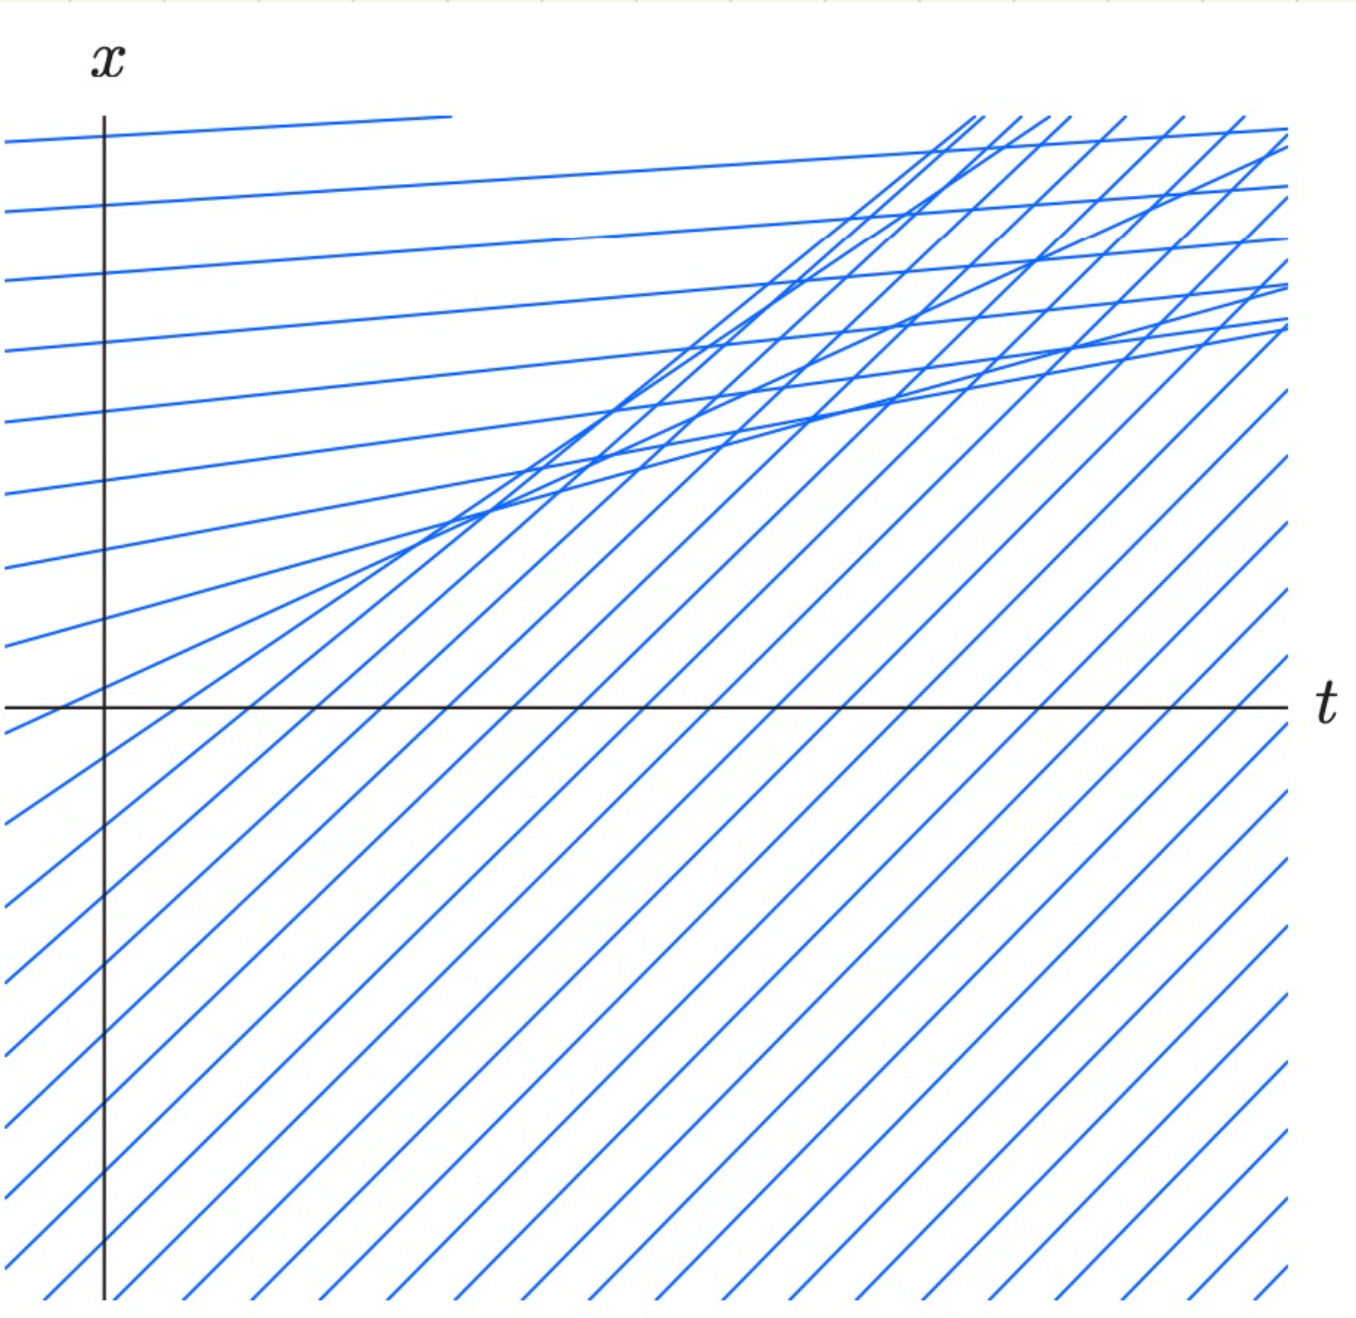
\includegraphics[height = 0.4\textwidth, width = 0.5\textwidth]{resource/cline.png}
	\caption{Characteristic lines for $
    u(0,x)=\frac{1}{2}\pi-tan^{-1}(x)
$ }
	\label{img:cline}
\end{figure}
Two characteristic lines that are not parallel must cross and the value of the solution is supposed to be equal the slope of the characteristic line passing through the point.\\
At a crossing point, the solution will have to be equal to two different values, one corresoponding to each characteristic line.\\
While mathematically, such a multiply valued solutions are possible, they are physically untenbale.\\
One needs to decide which (if any) of the possible values is the physically appropriate.\\
\end{example}
\subsection{The wave equation:d'Alembert's formula}
Let us consider the 1D wave equation:
\begin{equation}
    \label{eq13} \pdv[2]{u}{t}=c^2\pdv[2]{u}{x}
\end{equation}
where c>0 is a given constant\\
the wave speed, the initial data are of the form:
\begin{equation}
    \label{eq14} u(0,x)=f(x),\pdv{u}{t}(0,x)=g(x)
\end{equation}
The initial value problem is to find a $ \mathbb{C}^2 $ function that solves \eqref{eq13} and satisfies \eqref{eq14}\\
In this section, we will consider only the 1D case posed on the whole line R\\
Let us define the wave operator:
$$
    \square =\pdv[2]{}{t}-c^2\pdv[2]{}{x}
$$ 
Thus the wave equation becomes:
$$
    \square u=0
$$
In analogy with the elementary factorization
$$
    t^2-c^2x^2=(t-cx)(t+cx)
$$ 
We can write 
$$
    \square=(\pdv{}{t}-c\pdv{}{x})(\pdv{}{t}+c\pdv{}{x})
$$
Now, if
\begin{equation}
     \label{eq15}(\pdv{}{t}+c\pdv{}{x})u=0
\end{equation}
then u is automatically a solution of the wave equation, because
$$
    \square u=(\pdv{}{t}-c\pdv{}{x})(\pdv{}{t}+c\pdv{}{x})u=0
$$
Clearly, \eqref{eq15} is a transport equation with constant wave speed c, and its solutions are traveling waves with speed c:
$$
    u(t,x)=p(\xi)=p(x-ct)
$$
where p is an arbitrary function.\\
If $ p\in \mathbb{C}^2,u(t,x) $ is a classical solution of the wave equation \eqref{eq13}.\\
The factorization of $ \square $ can be written in the reverse order:
$$
    \square=(\pdv{}{t}+c\pdv{}{x})(\pdv{}{t}-c\pdv{}{x})
$$
Solving the transport equation:
$$
    (\pdv{}{t}-c\pdv{}{x})u=0
$$
with -c instead of c, we get:
$$
    u(t,x)=q(x+ct)
$$ 
where q is an arbitrary function.\\
the solution represent traveling waves moving to the left with constant speed c>0\\
If $ q\in \mathbb{C}^2$, we get a second family of solutions to the wave equation.\\
Thus there are both left and right traveling-wave solution,\\
Thus, we have two families of solutions of the wave equation:
\begin{align*}{}{}
u(t,x)&=p(x-ct)\\
u(t,x)&=q(x+ct), \forall p,q\in \mathbb{C}^2
\end{align*}
Any linear combination of these solutions is still a solution of \eqref{eq13}:
$$
    u(t,x)=p(x-ct)+q(x+ct),c>0
$$ 
\begin{theorem}[]{}
Every solution to \eqref{eq13} can be written in the form \begin{equation}
    \label{eq16} u(t,x)=p(x-ct)+q(x+ct), \forall p,q\in \mathbb{C}^2
\end{equation}
\end{theorem}
\textbf{Proof:}
\begin{align*}{}{}
    \xi &=x-ct\\
    \eta&=x+ct\\
    x=\frac{\xi+\eta}{2}&,t=\frac{\eta-\xi}{2c}\\
    u(t,x)&=u(\frac{\eta-\xi}{2c},\frac{\xi+\eta}{2})\\
    \text{so, }u(t,x)&=v(\xi,\eta)\\
    \text{Lets find a PED for v: }\\
    \pdv{u}{t}&=c(-\pdv{v}{\xi}+\pdv{v}{\eta})\\
    \pdv[2]{u}{t}&=c^2(\pdv[2]{v}{\xi}-2\pdv{v}{\xi}{\eta}+\pdv[2]{v}{\eta})\\
    \pdv[2]{u}{x}&=c^2(\pdv[2]{v}{\xi}+2\pdv{v}{\xi}{\eta}+\pdv[2]{v}{\eta})\\
    0&=\square u=\pdv[2]{u}{t}-c^2\pdv[2]{u}{x}\\
    &=-4c^2\pdv{v}{\xi}{\eta}=0\\
    \Leftrightarrow \pdv{v}{\xi}{\eta}&=0\\
    \frac{\partial}{\partial \xi}\frac{\partial v}{\partial \eta}v&=0\\
    \Leftrightarrow \frac{\partial w}{\partial \xi}&=0\\
    \Leftrightarrow w(\xi,\eta)&=w(\eta)\\
    \Leftrightarrow w=r(\zeta )\\
    \text{where } \zeta \text{ is an arbitary function of }\eta\\
    w=\pdv{v}{\eta}=r(\zeta )\\
    \text{Integrating we get: }\\
\end{align*}
Now we want to solve the initial value problem \eqref{eq16}:
\begin{align*}{}{}
u(t,x)&=p(x-ct)+q(x+ct)\\
u(0,x)&=p(x)+q(x)=f(x)\\
\pdv{u}{t}(0,x)&=-cp'(x)+cq'(x)=g(x)\\
&\begin{cases}
    p'(x)+q'(x)&=f(x)\\
    -cp'(x)+cq'(x)&=g(x)
\end{cases}\\
2p'(x)&=f(x)+\frac{g(x)}{c}\\
p(x)&=\frac{1}{2}f(x)-\frac{1}{2c}\int_{0}^{x}g(z)dz+a\\
&\text{where a is an integration constant}\\
q(x)&=f(x)-p(x)\\
&=\frac{1}{2}+\frac{1}{2c}\int_{0}^{x}g(z)dz-a\\
u(t,x)&=p(\xi)+q(\eta)\\
&=\frac{f(\xi)+f(\eta)}{2}-\frac{1}{2c}\int_{0}^{\xi}g(z)dz+\frac{1}{2c}\int_{0}^{\eta}g(z)dz\\
&=\frac{f(\xi)+f(\eta)}{2}+\frac{1}{2c}\int_{\eta}^{\xi}g(z)dz
\end{align*}
\textbf{This is called d'Alembert's solution to the IVP \eqref{eq14}}
\begin{theorem}[d'Alembert's solution]{}
The solution of the problem:
\begin{align*}{}{}
\pdv[2]{u}{t}&=c^2\pdv[2]{u}{x}\\
u(0,x)&=f(x)\\
\pdv{u}{t}(0,x)&=g(x),x\in \mathbb{R}
\end{align*}
is given by:
$$
    u(t,x)=\frac{f(x+ct)+f(x-ct)}{2}+\frac{1}{2c}\int_{x-ct}^{x+ct}g(z)dz, \forall f\in \mathbb{C}^2, g\in \mathbb{C}^1
$$ 
Note that this formula provides a classical solution if $ f\in \mathbb{C}^2 $ and $ g\in \mathbb{C}^1 $ 
\end{theorem}
\textbf{External forcing:}
\\If a homogeneuous medium is subject to an external force F, then the system is described as:
\begin{equation}
   \label{eq17} \pdv[2]{u}{t}=c^2\pdv[2]{u}{x}+F(x,t)
\end{equation}
We apply a generalized version of d'Alembert's technique. To simplify,we first impose homogeneuous initial data:
\begin{align*}{}{}
u(0,x)&=0\\
\pdv{u}{t}(0,x)&=0\\
\end{align*}
We search for a solution in the form  $ u(t,x)=v(\xi,\eta) $ and from the chain rule,we get
\begin{align*}{}{}
\pdv{v}{\xi}{\eta} &=\frac{1}{-4c^2}F(\frac{\eta-\xi}{2c},\frac{\eta+\xi}{2})
\end{align*}
Intergrating with respect to $ \eta $, we get
$$
    \pdv{v}{\xi}(\xi,\eta)-\pdv{v}{\xi}(\xi,\xi)=\frac{1}{-4c^2}\int_{\xi}^{\eta}F(\frac{\zeta-\xi}{2c},\frac{\zeta+\xi}{2})d\zeta
$$ 
From the identities:
$$
    \pdv{u}{t}=c(-\pdv{v}{\xi}+\pdv{v}{\eta}),\pdv{u}{x}=c(\pdv{v}{\xi}+\pdv{v}{\eta})
$$ 
We get:
\begin{align*}{}{}
\pdv{v}{\xi}(\xi,\eta)=-\frac{1}{2c}\pdv{u}{t}(\frac{\eta-\xi}{2},\frac{\eta+\xi}{2})+\frac{1}{2c}\pdv{u}{x}(\frac{\eta-\xi}{2},\frac{\eta+\xi}{2})\\
\end{align*}
Taking $ \xi=\eta $ :
$$
    \pdv{v}{\xi}(\xi,\xi)=-\frac{1}{2c}\pdv{u}{t}(0,\xi)+\frac{1}{2c}\pdv{u}{x}(0,\xi)=0
$$ 
because of homogeneuous initial conditions. Thus \eqref{eq17} becomes:
$$
    \pdv{v}{\xi}(\xi,\eta)=\frac{1}{-4c^2}\int_{\xi}^{\eta}F(\frac{\zeta-\xi}{2c},\frac{\zeta+\xi}{2})d\zeta
$$ 
Now, we integrate this with respect to $ \xi $:
\begin{align*}{}{}
-v(\xi,\eta)=v(\eta,\eta)-v(\xi,\eta)=\frac{1}{-4c^2}\int_{\xi}^{\eta}\int_{\xi}^{\zeta}F(\frac{\zeta-\xi}{2c},\frac{\zeta+\xi}{2})d\zeta d\xi\\
\end{align*}
since $ v(\xi,\xi)=0 $, Thus:
\begin{align*}{}{}
v(\xi,\eta)&=\frac{1}{4c^2}\int_{\xi}^{\eta}\int_{\phi}^{\zeta}F(\frac{\zeta-\phi}{2c},\frac{\zeta+\phi}{2})d\zeta d\phi\\
&=\frac{1}{4c^2}{\iint}_{T(\xi,\eta)}F(\frac{\zeta-\phi}{2c},\frac{\zeta+\phi}{2})d\zeta d\phi\\
\end{align*}
That is the double integral takes place over the triangle$$
    T(\xi,\eta)=\{(\phi,\zeta):\xi\leq\phi\leq\zeta\leq\eta\}
$$ 
Recalling that $ \xi=x-ct $ and $ \eta=x+ct $ and setting $ \phi=y-cs $ and $ \zeta=y+cs $,
the inequality $ \xi\leq\phi\leq\zeta\leq\eta $   becomes $ x-ct\leq y-cs\leq y+cs\leq x+ct $, \\
So T($ \xi,\eta $) cna be rewritten as $ D(t,x)=\{(s,y)|x-c(t-s)\leq y\leq x+c(t-s),0\leq s\leq t\} $ 
\begin{figure}[H]
    \centering
    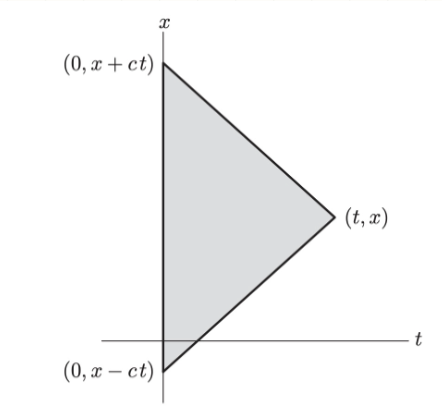
\includegraphics[height = 0.4\textwidth, width = 0.5\textwidth]{resource/4.png}
    \caption{The Domain of integration $ D(t,x) $}
\end{figure}
Using the change of variables $ \frac{\zeta-\phi}{2c}=s $ and $ \frac{\zeta+\phi}{2}=y $ for the double integrals and computing the Jacobian, we get:
$\det$
$\begin{pmatrix}
\pdv{\phi}{y} & \pdv{\phi}{s} \\
\pdv{\zeta}{y} & \pdv{\zeta}{s}
\end{pmatrix}$ $=\det$
$\begin{pmatrix}
1 & -c \\
1 & c
\end{pmatrix}$ $=2c$
\\Thus,
\begin{align*}{}{}
u(t,x)&=\frac{1}{2c}\iint_D(t,x)F(s,y)dsdy\\
&=\frac{1}{2c}\int_{0}^{t}\int_{x-c(t-s)}^{x+c(t-s)}F(s,y)dyds
\end{align*}
is the formula for the solution to the forced wave equation with homogeneuous initial conditioni.\\
To solve the case of general initial condition, one needs to take the sum of the solution to the forced equation with homogeneuous initial conditions plus the d'Alembert solution to the unforced equation subject to inhomogeneuous boundary conditions.\\
\section{Lecture 4 (02-12)}
\begin{theorem}[]{}
The solution of the problem:
$$
    \begin{cases}
        \pdv[2]{u}{t}=c^2\pdv[2]{u}{x}+F(x,t)\\
        u(0,x)=f(x)\\
        \pdv{u}{t}(0,x)=g(x)
    \end{cases}
$$ is given by
\begin{align*}{}{}
u(t,x)&=\frac{f(x-ct)+f(x+ct)}{2}+\frac{1}{2c}\int_{x-ct}^{x+ct}g(z)dz+\frac{1}{2c}\int_{0}^{t}\int_{x-c(t-s)}^{x+c(t-s)}F(s,y)dyds
\end{align*}
The triangle D(t,x) is called the domain of dependence of the point (t,x)
\end{theorem}
\begin{example}[]{}
 $$
    \pdv[2]{u}{t}=c^2\pdv[2]{u}{x}+sin\omega tsinx,u(0,x)=0,\pdv{u}{t}(0,x)=0
 $$ 
 So:\begin{align*}{}{}
 F(t,x)&=sin\omega tsinx\\
 u(t,x)&=\frac{1}{2c}\int_{0}^{t}\int_{x-t+s}^{x+t-s}sin\omega ssinydyds\\
 &=\frac{1}{2}\int_{0}^{t}sin\omega s[cos(x-t+s)-cos(x+t-s)]ds\\
 &=\begin{cases}
    \frac{sin\omega t -\omega sint}{1-\omega^2}sinx, \omega\neq 1\\
    \frac{sint-tcost}{2}sinx, \omega=1
 \end{cases}
 \end{align*}
 When $ \omega\neq1 $ ,the solution is bounded.
 \\If $ \omega \in Q $ ,then the solution u is periodic in time.\\
 If $ \omega \in I $ ,then u is quasi-periodic(it never exactly repeats) in time.  \\
 When $ \omega=1 $ the solution is unbounded. 
\end{example}
\subsection{Exercises}
 \begin{enumerate}[label=\circled{\arabic*}] 
 \item Supposed u(t,x) is defined for all $(t,x)\in R^2$ and solves $\pdv{u}{t}+2u=0.$\\
 Prove that $ \lim_{t\rightarrow+\infty}u(t,x)=0  $ for all x \\
 SOL:
 \begin{align*}{}{}
 u(0,x)=f(x)\\
 u(t,x)=e^{-2t}f(x)\\
 \lim_{t\rightarrow+\infty}u(t,x)=0
 \end{align*}
 \item Let u(t,x) solve the initial value problem $\pdv{u}{t}+u^c=0,u(0,x)=f(x)  $, where f(x) is a bounded $ \mathbb{C}^1 $ function of $ x\in\mathbb{R} $ \\
 (a): show that if $f(x)\geq 0$ for all x, then u(t,x) is defined for all $ t>0 $, and $ \lim_{t\rightarrow+\infty}u(t,x)=0 $\\
 (b): On the other hand , if $ f(x)<0 $ , then the solution u(t,x) is not defined for all t>0, but in fact, $ \lim_{t\rightarrow r^{-}}u(t,x)=-\infty,\text{ for some }0<r<\infty $
 Given x , what is the corresoponding value of r?\\
 (c):Given f(x) as in part (b), what is the longest time interval $ 0<t<t_\star $ on which u(t,x) is defined for all $ x\in \mathbb{R} $?
\\SOL:
\begin{align*}{}{}
\pdv{u}{t}&=-u^2,u(0,x)=f(x)\\
\frac{du}{u^2}&=-dt\Rightarrow -\frac{1}{u}=-t-c(x)\\
\frac{1}{u}&=t+c(x)\Rightarrow u(t,x)=\frac{1}{t+c(x)}\\
u(0,x)&=f(x)=\frac{1}{c(x)}\\
u(t,x)&=\frac{1}{t+\frac{1}{f(x)}}=\frac{f(x)}{tf(x)+1}\\
(a):&f(x)\geq 0\Rightarrow u(t,x) \text{ is defined for any }t\geq0 \text{ and } \lim_{t\rightarrow+\infty}u(t,x)=0\\
(b):&f(x)<0\Rightarrow \tau(x)=\frac{1}{f(x)} \Rightarrow u(t,x)=\frac{1}{t+\tau(x)}\\ 
(c): &If f(x)<0,[0,\tau(x))\\
t_\star&=\inf\{\tau(x):x\in \mathbb{R}\}=inf_{x\in \mathbb{R}}-\frac{1}{f(x)}=-\frac{1}{inf_{x\in \mathbb{R}}f(x)}\\
\text{So we can have } f(x)&=tan^{-1}(x)\\
\end{align*}     
\item Solve the following initial value problem and graph the solution at times t=1,2,and 3:\\
(a) $u_t-3u_x=0,u(0,x)=e^{-x^2}$
\\Recall:\begin{align*}{}{}
\pdv{u}{t}+c\pdv{u}{x}&=0\\
\text{We knnow that } u(t,x)&=v(\xi)=(x-ct)\\
\forall v&\in \mathbb{C}^1\\
u(0,x)&=f(x)=v(x)\\
\text{Thus }u(t,x)&=f(x-ct)\\
\end{align*}
\textbf{In our case:}
\begin{align*}{}{}
u(t,x)=f(x+3t)&=e^{-(x+3t)^2}\\
\end{align*}
\item Graph some of the characteristic lines for the following equations and write down a formula for the general solution:
\\(a)$u_t-3u_x=0$,
\\SOL: The characteristic lines of the equation $\pdv{u}{t}+c(x) \pdv{u}{x}=0$ are the solution of the ODE:$$
    \dv{x}{t}=c(x)
$$ 
In our case $ \dv{x}{t}=-3 \rightarrow x(t)=-3t+k $ 
\item (a)Prove that if the initial data is bounded,$|f(x)| \leq M $ for all $ x\in\mathbb{R} $,then the solution to the damped transport equation $\pdv{u}{t}+c\pdv{u}{x}+au=0 $ with a>0 satisfies $ u(t,x)\rightarrow 0 $ as $ t\rightarrow\infty $  
\\(b) Find a solution to it that is defined for all (t,x) but does not satisfy $ u(t,x)\rightarrow0 $ as $ t\rightarrow +\infty $  
\\SOL: Recall the solution to it with initial condition u(0,x)=f(x) is given by \begin{align*}{}{}
u(t,x)&=f(x-ct)e^{-at}\\
|u(t,x)|&=|f(x-ct)|e^{-at}\leq Me^{-at}\\
\text{(b) }f(x)&=e^{Ax}\\
u(t,x)&=e^{A(x-ct)-at}=e^{-(Ac+a)t+Ax}\\
\text{Choose }A\leq -\frac{a}{c}
\end{align*}
\item (a) Write down a formula for the general solution to the nonlinear partial differential equation $u_{t}+u_{x}+u^{2}=0$. \\
(b) Show that if the initial data is positive and bounded, $0\leq u(0,x)=f(x)\leq M$, then the solution exists for all $t>0$, and $u(t,x)\rightarrow 0$ as $t\rightarrow \infty$. \\
(c) On the other hand, if the initial data is negative somewhere, so $f(x)<0$ at some $x\in\mathbb{R}$, then the solution blows up in finite time: $\lim_{t\rightarrow\tau^{-}}u(t,y)=-\infty$ for some $\tau>0$ and some $y\in\mathbb{R}$.\\
(d) Find a formula for the earliest blow-up time $\tau_{*}>0$.
\\SOL: Writing u(t,x) in terms of the characteristic variable $\xi=x-t$ we get:
$$
    u(t,x)=v(t,\xi)=u(t,\xi+t)
$$ 
Let us find the equation for v:
\begin{align*}{}{}
\pdv{v}{t}&=\pdv{u}{t}+\pdv{u}{x}=-u^2=-v^2\\
\Rightarrow \frac{dv}{v^2}&=-dt \Rightarrow -\frac{1}{v}=-t-c(\xi)\\
\Rightarrow v(t,\xi)&=\frac{1}{t+c(\xi)}\\
\Rightarrow u(t,x)&=\frac{1}{t+c(x-t)}\\
\end{align*}
Where c is an arbitrary $ \mathbb{C}^1 $ function.\\
(b): if there is an initial condition $ u(0,x)=f(X) $, then we can determinec(x):\begin{align*}{}{}
u(0,x)&=f(x)=\frac{1}{c(x)}\\
\Rightarrow u(t,x)&=\frac{1}{t+\frac{1}{f(x-t)}}=\frac{f(x-t)}{tf(x-t)+1}\\
\end{align*} 
If $ 0\leq f(x) $, then $ tf(x-t)+1\neq0 $,so u(t,x) id defined for any t>0.\\
The function $ \frac{s}{ts+1} $ is increasing in s\\
Therefore:$$
    0\leq  u(t,x)\leq \frac{M}{Mt+1}\underbrace{\rightarrow}_{(\text{as } t\rightarrow\infty)} 0 \text{ as } f(x)\leq M
$$   
(c): The solution formula implies that, if $ f(x)<0 $ then\begin{align*}{}{}
u(t,x_\star)&\rightarrow-\infty \\
\text{ as } t\rightarrow\tau&=-\frac{1}{f(x)}\\
where x_\star&=x-\frac{1}{f(x)}
\end{align*} 
(d): $$
    \tau_{*}=-\frac{1}{\inf_{x\in \mathbb{R}}f(x)}
$$ 
\end{enumerate}
\section{Lecture 5 (02-17)-Exercise}
\subsection*{Problem 1}
2.2.17. (a) Solve the initial value problem $u_t - xu_x = 0$, $u(0,x) = (x^2 + 1)^{-1}$.  
(b) Graph the solution at times $t=0,1,2,3$.  
(c) What is $\lim_{t \to \infty} u(t,x)$?
\begin{solution}
   (a)\\ (1) find characteristic curves by solving$$
        \dv{x}{t}=-x
    $$
    \begin{align*}{}{}
    x(t)=x_0e^{-t}
\end{align*}
    (2) find u from the information that u(t,x) is constant along the characteristics:$$
        u(t,x(t))=u(0,x(0))=f(x(0))
    $$  
    \begin{align*}{}{}
    u(t,x_0e^{-t})&=f(x_0)=\frac{1}{x_0^2+1}\\
    \text{Denote } x&=x_0e^{-t}\Rightarrow x_0=e^tx\\
    u(t,x)&=\frac{1}{e^{2t}x^2+1}\\
    &=\frac{e^{-2t}}{x^2+e^{-2t}}\\
    \end{align*}
(b)t=0,1,2,3\\
(c) $ \lim_{t\rightarrow+\infty}u(t,x)=\begin{cases}
    0, x\neq 0\\
    1, x=0
\end{cases} $ 
\end{solution}
\subsection*{Problem 2}
2.2.25. Suppose that $c(x) \in C^1$ is continuously differentiable for all $x \in \mathbb{R}$. (a) Prove that the characteristic curves of the transport equation (2.16) cannot cross each other. (b) A point where $c(x_*) = 0$ is known as a fixed point for the characteristic equation $\frac{dx}{dt} = c(x)$. Explain why the characteristic curve passing through a fixed point $(t, x_*)$ is a horizontal straight line. (c) Prove that if $x = g(t)$ is a characteristic curve, then so are all the horizontally translated curves $x = g(t + \delta)$ for any $\delta$. (d) True or false: Every characteristic curve has the form $x = g(t + \delta)$, for some fixed function $g(t)$. (e) Prove that each non-horizontal characteristic curve is the graph $x = g(t)$ of a strictly monotone function. (f) Explain why a wave cannot reverse its direction. (g) Show that a non-horizontal characteristic curve starts, in the distant past, $t \to -\infty$, at either a fixed point or at $-\infty$ and ends, as $t \to +\infty$, at either the next-larger fixed point or at $+\infty$.
\begin{solution}
(a)\\
$$\dv{x}{t}=c(x),x(t_0)=x_0$$
If $ x_1(t),x_2(t) $ are characteristic curves that cross each other at $ (t_0,x_0) $   then they both solve the same Cauchy problem.
\\By uniqueness, we have $ x_1(t)=x_2(t) $ for all t
\\(b)\\
We know that $ x_\star $ is a zero of C:$ C(x_\star)=0 $ Let's consider the following problem:$$
    \begin{cases}
        \dv{x}{t}=c(x)\\
        x(0)=x_\star
    \end{cases}
$$  
So, $ x(t)=x_\star $\\
(c) \\
If g(t) is a characteristic curve$$
    \frac{d}{dt}g(t)=c(g(t))
$$ 
Then \begin{align*}{}{}
g(t+\delta)=g_\delta(t) \text{ is also characteristic}\\
\end{align*}
since it satisfies $$
    \frac{d}{dt}g_\delta(t)=c(g_\delta(t))
$$ since c does not depend on t
\\(d)\\
False: If c admit a zero and $c\neq 0$,then $ \exists $ single g such that any characteristicis of the form $ g(t+\delta) $.\\
In deed, the fixed point solution and non-fixed point solutioins are not given with the same g.  
\\(e)\\
To determine the monotonicity of g, we need to check the sign of g'(t).\\
it is always >0 or<0 in between the horizontal lines.\\
Then g'(t)=c(g(t)).\\
If $ \exists t_1 \text{ and }t_2$ so that $ g'(t_1)>0 \text{ and }g'(t_2) <0$ then $ \exists t_\star$ between $ t_1,t_2 $ s,t, $c(g(t_\star)) $=0, therefore x(t) is a fixed point solution and the graph should be a horizontal line\\
(f)\\
c(x(t)) is the soeed of the wave   \\
Reformultion: Can the function c(x(t)) change its sign along a fixde characteristic curve?\\
If c(x(t1)>0),c(x(t2))<0, then exists $c(x(t_\star)) $=0, therefore x(t) is a fixed point solution and the graph should be a horizontal line\\
(g)\\

\end{solution}
\subsection*{Problem 3}
2.4.11.(a) Write down an explicit formula for the solution to the initial value problem
$$\frac{\partial^2 u}{\partial t^2} - 4 \frac{\partial^2 u}{\partial x^2} = 0, \quad u(0,x) = \sin x, \quad \frac{\partial u}{\partial t}(0,x) = \cos x, \quad -\infty < x < \infty, \quad t \geq 0.$$

(b) True or false: The solution is a periodic function of $t$.

(c) Now solve the forced initial value problem
$$\frac{\partial^2 u}{\partial t^2} - 4 \frac{\partial^2 u}{\partial x^2} = \cos 2t, \quad u(0,x) = \sin x, \quad \frac{\partial u}{\partial t}(0,x) = \cos x, \quad -\infty < x < \infty, \quad t \geq 0.$$

(d) True or false: The forced equation exhibits resonance. Explain.

(e) Does the answer to part (d) change if the forcing function is $\sin 2t$?
\begin{solution}
    (a)\begin{align*}{}{}
    u(t,x)&=\frac{sin(x-2t)+sin(x+2t)}{2}+\frac{1}{4}(sin(x+2t)-sin(x-2t))\\
    &=\frac{1}{4}sin(x-2t)+\frac{3}{4}sin(x+2t)
    \end{align*}
    (b)\\
    T s.t. u(t+T,x)=u(t,x)\\
    $T=\pi$\\
    (c)\\
    \begin{align*}{}{}
    u(t,x)&=\frac{1}{4}sin(x-2t)+\frac{3}{4}sin(x+2t)+\frac{1}{4}\sum_{0}^{t}\sum_{x-2(t-s)}^{x+2(t-s)}cos2sdyds\\
    &=\frac{1}{4}sin(x-2t)+\frac{3}{4}sin(x+2t)+\frac{1}{4}(1-cos2t)
    \end{align*}
    (d)\\
    resonance:unbounded\\
    False, no resonance since the solution is bounded
\end{solution}
\subsection*{Problem 4}
2.4.13. Let $u(t,x)$ be a classical solution to the wave equation $u_{tt}=c^2 u_{xx}$. The total energy 
$$E(t) = \int_{-\infty}^{\infty} \frac{1}{2} \left[ \left( \frac{\partial u}{\partial t} \right)^2 + c^2 \left( \frac{\partial u}{\partial x} \right)^2 \right] dx$$
represents the sum of kinetic and potential energies of the displacement $u(t,x)$ at time $t$. Suppose that $\nabla u \to 0$ sufficiently rapidly as $x \to \pm \infty$; more precisely, one can find $\alpha > \frac{1}{2}$ and $C(t) > 0$ such that $|u_t(t,x)|, |u_x(t,x)| \leq C(t)/|x|^{\alpha}$ for each fixed $t$ and all sufficiently large $|x| \gg 0$. For such solutions, establish the Law of Conservation of Energy by showing that $E(t)$ is finite and constant. Hint: You do not need the formula for the solution.
\begin{solution}
    We need to show that $ \dv{E(t)}{t}=0 $ 
    \begin{align*}{}{}
    \frac{d}{dt}E(t)&=\frac{d}{dt}\int_{-\infty}^{+\infty}\frac{1}{2}[(\pdv{u}{t})^2+c^2(\pdv{u}{x})^2]dx\\
    &=\int_{-\infty}^{+\infty}[(\pdv{u}{t})\cdot\pdv[2]{u}{t}+c^2(\pdv{u}{x})\pdv{u}{x}{t}]dx\\
    &=c^2\int_{-\infty}^{+\infty}[(\pdv{u}{t})\cdot\pdv[2]{u}{x}+(\pdv{u}{x})\pdv{u}{x}{t}]dx\\
    &=c^2\int_{-\infty}^{+\infty}1\cdot \frac{\partial}{\partial x}(\pdv{u}{t}\cdot \pdv{u}{x})dx \text{ integration by parts}\\
    &=-c^2\int_{-\infty}^{+\infty} \underbrace{\frac{\partial}{\partial x}1}_{=0}\cdot(\pdv{u}{t}\cdot \pdv{u}{x})dx +0 (\text{boundary terms})\\
    &=0
    \end{align*}
\end{solution}
\section{Lecture 6 (02-19)--{Fourier Series}}
\subsection*{Problem 5}
2.4.15
\begin{solution}
    \begin{align*}{}{}
    E(t)&=\int_{-\infty}^{+\infty} \left[ \left( \frac{\partial u}{\partial t} \right)^2 + c^2 \left( \frac{\partial u}{\partial x} \right)^2 \right]dx\\
    \dv{E(t)}{t}&=\int_{-\infty}^{+\infty}[\pdv{u}{t}\cdot \pdv[2]{u}{t}+c^2\pdv{u}{x}\cdot \pdv{u}{x}{t}]dx\\
    &=\int_{-\infty}^{+\infty}[c^2(\pdv{u}{t}\cdot \pdv[2]{u}{x}+\pdv{u}{x}\cdot \pdv{u}{x}{t})-a(\pdv{u}{t})^2]dx\\
    &=c^2\int_{-\infty}^{+\infty}1\cdot \frac{\partial}{\partial x}(\pdv{u}{x}\cdot \pdv{u}{t})dx- a\sum_{-\infty}^{+\infty}(\pdv{u}{t})^2dx\\
    &\leq 0 \Leftrightarrow \dv{E(t)}{t}\leq 0\\
    \text{So, } E(t) \text{ is decreasing}
    \end{align*}
    We need to prove that there is a unique solution to the problem$\begin{cases}
    \pdv[2]{u}{t}+a\pdv{u}{t}=c^2\pdv[2]{u}{x}\\
    u(0,x)=f(x)\\
    \pdv{u}{t}(0,x)=g(x)
    \end{cases}$
    Suppose $ \exists u_1(t,x),u_2(t,x)$\begin{align*}{}{}
    u(t,x)=u_1(t,x)-u_2(t,x)\\
    \end{align*}  
    u satisfies the equation with initial data$$
        u(0,x)=\pdv{u}{t}(0,x)=0
    $$ 
    We need to show that $ u(t,x)=0  \forall  t 0,x  $$$
        E(0)=\int_{-\infty}^{+\infty}(\pdv{u}{t}(0,x))^2+c^2(\pdv{u}{x}(0,x))^2dx=0
    $$ 
    Since E(0)=0, $ \dv{E(t)}{t}\leq0 ,E(t\geq0) \Rightarrow E(t)=0$ 
    $ \Rightarrow \pdv{u}{t}(t,x)=\pdv{u}{x}(t,x)=E,\forall x,t \Rightarrow u \text{ is constant } \Rightarrow u(t,x)=0$ 
\end{solution}
\subsection*{Problem 6}
2.4.17
\begin{solution}
    \begin{align*}{}{}
    \square&= \pdv[2]{t}-c^2(x)\pdv[2]{x}\\
    (\pdv{t}+c(x)\pdv{x})(\pdv{t}-c(x)\pdv{x})&=\pdv[2]{t}-c^2(x)\pdv[2]{x}-c(x)c'(x)\pdv{x}\\
    \end{align*}
    since $ c'(x)\neq 0 $, the d'Alembert formula does not apply
\end{solution}
\subsection{Fourier Series}
The linear heat equation:
\begin{equation}
    \label{eq18}\begin{cases}
\pdv{u}{t}=\pdv[2]{u}{x}\\
     \pdv{u}{t}=L[u]
\end{cases}
\end{equation}
\begin{align*}{}{}
L[u]&=\pdv[2]{u}{x}
\\L[u+v]&=L[u]+L[v]\\
L[\alpha u]&=\alpha L[u]
\end{align*}
These are true for any functions u and v in $ \mathbb{C}^2 $ \\
Let us find solutions to  \eqref{eq18} in the form.$$
    u(t,x)=e^{\lambda t}v(x)
$$ 
\begin{align*}{}{}
\pdv{u}{t}&=\pdv{t}[e^{\lambda t}v(x)]\\
&=\lambda e^{\lambda t}\\
L[u]&=L[e^{\lambda t }v]\\
&=\pdv[2]{x}[e^{\lambda t }v]\\
&=e^{\lambda t}\pdv[2]{x}v\\
&=e^{\lambda t}L[v]\\
\pdv{u}{t}&=L[u]\\
\end{align*}
Thus $ u=e^{\lambda t}v $ will be a solution to \eqref{eq18} iff $$
    L[v]=v''=\lambda v
$$ 
\begin{align*}{}{}
\pdv{u}{t}=\pdv[2]{u}{x},x\in \mathbb{R}
\end{align*}
Any nonzero linear combination of these particular solutions is still a solution of \eqref{eq18}\\
For example$$
    u(t,x)=c_1e^{-t}\cos{x}+c_2e^{-4t}\sin{2x}+c_3x+c_4
$$ The heated ring
\begin{align*}{}{}
\pdv{u}{t}&=\pdv[2]{u}{x}\\
u(t,-\pi)&=u(t,\pi)\\
\pdv{u}{x}(t,-\pi)&=\pdv{u}{x}(t,\pi)\\
u(0,x)&=f(x)\\
u(t,x)&=e^{\lambda t}v(x)\\
v''&=\lambda v\\
v(-\pi)&=v(\pi),v'(-\pi)=v'(\pi)\\
\end{align*}
find $ \lambda $ and v(x)\\
case 1: $ \lambda=\omega^2>0 $\\
\begin{align*}{}{}
v(x)&=ae^{\omega x}+be^{-\omega x},\forall a,b\in\mathbb{R}\\
ae^{\omega \pi}+be^{-\omega \pi}&=ae^{-\omega \pi}+be^{\omega \pi}\\
a\omega e^{-\omega \pi}-b\omega e^{\omega \pi}&=a\omega e^{\omega \pi}-b\omega e^{-\omega \pi}\\
\omega &\neq0\\
e^{\omega \pi}(b-a)+(a-b)e^{-\omega \pi}&=0\\
(e^{\omega \pi}-e^{-\omega \pi})(b-a)&=0\\
\Leftrightarrow \underbrace{(e^{2\omega \pi}-1)}_{\neq 0}(b-a)&=0\\
\Rightarrow a&=b \text{ and } a=-b\\
\Rightarrow a=b&=0 \Rightarrow v(x)=0
\end{align*}
case 2: $ \lambda=0 $\\
\begin{align*}{}{}
v''&=0\\
v(x)=a+bx,\forall a,b\in\mathbb{R}\\
a-b\pi&=a+b\pi\\
\Rightarrow b&=0,\forall a\in \mathbb{R}\\
\text{Thus } v(x)&=a\\
u(t,x)&=e^{\lambda t}v(x)=a
\end{align*}
case 3: $ \lambda=-\omega^2<0 $\\
\begin{align*}{}{}
v''&=\lambda v\\
v(x)&=a\cos{\omega x}+b\sin{\omega x},\forall a,b\in\mathbb{R}\\
a\cos{\omega \pi}-b\sin{\omega \pi}&=a\cos{\omega \pi}+b\sin{\omega \pi}\\
a\sin{\omega \pi}+b\cos{\omega \pi}&=-a\sin{\omega \pi}+b\cos{\omega \pi}\\
2b\sin{\omega \pi}&=0,2a\sin{\omega \pi}=0\\
\text{If } \sin{\omega \pi}&\neq0 \\
\text{then } a&=b=0\text{ If } \sin{\omega \pi}= 0 \\
 \Rightarrow \forall a, b\in \mathbb{R}, \omega&=1,2,\cdots \\
 v(x)&=a\cos{kx}+b\sin{kx} \forall a,b\in \mathbb{R}\\
 \text{With } \lambda&=-k^2\\
 u_k(t,x)&=e^{-k^2t}(\cos{kx})\\
 u'_k(t,x)&=e^{-k^2t}(\sin{kx})\\
\end{align*}
By Fourier:
\begin{align*}{}{}
u(t,x)=\frac{a_0}{2}+\sum_{k=1}^{\infty}[a_ke^{-k^2t}\cos{kx}+b_ke^{-k^2t}\sin{kx}]\\
\end{align*}
With coefficients $ a_k,b_k $,the parameters $ a_k,b_k $ are fixed such that$$
    u(0,x)=f(x)
$$ 
\subsection{Fourier Series 2}
We introduce $ L^2 $-inner product for continuous functions on the interval $ [-\pi.\pi] $  
$$
    <f,g>=\frac{1}{\pi}\int_{-\pi}^{\pi}f(x)g(x)dx
$$ 
Basic properties of the inner product:
\begin{itemize}
\item symmetry: $ <f,g>=<g,f> $
\item bilinearity: $ <\alpha f_1+\beta f_2,g>=\alpha<f_1,g>+\beta<f_2,g> $
\item positivity: $ <f,f> > 0 \text{ if } f\neq0 ,\text{ and } <0,0>=0 $
\end{itemize}
The associated norm ($ L^2 $-norm) is defined by $$ ||f||=\sqrt{<f,f>} $$
\begin{lemma}[]{}
The trigonometric functions $ 1,\cos{x},\sin{x},\cos(2x),\sin(2x),\cdots $ 
satisfies the relations \begin{align*}{}{}
<\cos(kx),\cos(lx)>&=<\sin(kx),\sin(lx)>=0,\forall k\neq l \text{ integers}\\
<\cos(ux),\sin(lx)>&=0,\forall u,l\\
||1||&=\sqrt{2}\\
||\cos(kx)||&=||\sin(kx)||=1,\forall k \neq0\\
f\perp g &\Leftrightarrow <f,g>=0
\end{align*}
\end{lemma}
\begin{align*}{}{}
f(x)&=\frac{a_0}{2}+\sum_{k=1}^{\infty}[a_k\cos{kx}+b_k\sin{kx}]\\
<f,\cos(lx)>&=\frac{a_0}{2}<1,\cos(lx)>+\sum_{k=1}^{\infty}[a_k<\cos{kx},\cos{lx}>+b_k<\sin{kx},\cos{lx}>]\\
&=a_l<\cos{lx},\cos{lx}>\\
&=a_l\\
b_l&=<f,\sin(lx)>
\end{align*}
\section{Lecture 7 (02-24)}
\begin{definition}[]{}
The Fourier series of a function $ f:[-\pi,\pi]\rightarrow\mathbb{R} $ is
$$
    f\approx \frac{a_0}{2}+\sum_{k=1}^{\infty}[a_k\cos{kx}+b_k\sin{kx}]
$$ where $ a_k=<f,\cos(kx)>,b_k=<f,\sin(kx)>,k=1,2,\cdots $ 
\end{definition}
\begin{example}[]{}
 \begin{enumerate}[label=\circled{\arabic*}] 
 \item f(x)=x
 \begin{align*}{}{}
 a_k=0,b_k=\frac{2}{k}(-1)^{k+1}\\
 \text{Therefore },x\approx 2(\sin{x}-\frac{1}{2}\sin{2x}+\frac{1}{3}\sin{3x}-\cdots)
 \end{align*}
 \end{enumerate}
\end{example}
\begin{definition}[Piecewise continuous function]{}
A function $ f:[a,b]\rightarrow\mathcal{R} $ is piecewise continuous if it is defined and countinuous except possibily at finite number of points 
\end{definition}
\begin{proposition}[even and odd function]{}
If f is even,then $ b_k=0 $ 
\\If f is odd, then $ a_k=0 $ 
\end{proposition}
\begin{example}[]{}
 \begin{enumerate}[label=\circled{\arabic*}] 
 \item \begin{align*}{}{}
 f(x)=|x|,\text{ even }\\
 a_k=\begin{cases}
    0, & \text{ if } k \text{ is even}\\
    -\frac{4}{\pi k^2}, & \text{ if } k \text{ is odd}
 \end{cases}
 \end{align*}
 by theorem, this series converges to the $ 2\pi $ periodic extension of |x|
 \begin{align*}{}{}
 \text{Let }x=0,\text{ we have}\\
 \frac{\pi^2}{8}=\sum_{k=0}^{\infty}\frac{1}{(2k+1)^2}
 \end{align*} 
 \item computing $ \sum_{k=1}^{\infty}\frac{1}{k^2}=S $
 \begin{align*}{}{}
 \frac{S}{4}&=\sum_{k=1}^{\infty}\frac{1}{(2k)^2}\\
 \frac{3}{4}S&=S-\frac{S}{4}=\sum_{k=0}^{\infty}\frac{1}{(2k+1)^2}=\frac{\pi^2}{8}\\
    S&=\frac{\pi^2}{6}
 \end{align*} 
 \end{enumerate}
\end{example}
\subsection{Complex Fourier series}
Euler formulas:
\begin{align*}{}{}
e^{-ikx}&=\cos(kx)-i\sin(kx)\\
\cos(kx)&=\frac{1}{2}(e^{ikx}+e^{-ikx})\\
\sin(kx)&=\frac{1}{2i}(e^{ikx}-e^{-ikx})
\end{align*}
For any $ f,g:[-\pi,\pi]\rightarrow C $ \\
$ L^2 $-Hermitian inner product defined by$$
    <f,g>=\frac{1}{2\pi}\int_{-\pi}^{\pi}f(x)\overline{g(x)}dx
$$  where $ \overline{g(x)} $ is the complex conjugate of g(x)\\
$ L^2 $-Hermitian norm is defined by$$
    ||f||=\sqrt{<f,f>}$$
Direct computation shows that$$
        <e^{ikx},e^{iex}>=\begin{cases}
            1, & \text{ if } k=e\\
            0, & \text{ if } k\neq e
        \end{cases}$$
and $$
    ||e^{ikx}||=1
$$ 
If f is a given continuous (or piecewise continuous) complex function\\
then$$
    f \approx \sum_{k=-\infty}^{\infty}c_ke^{ikx}
$$ with $ c_k=<f,e^{ikx}> $
\\It is easy to see that\begin{align*}{}{}
a_k&=c_k+c_{-k}\\
b_k&=i(c_k-c_{-k})\\
c_k&=\frac{1}{2}(a_k-ib_k)\\
c_{-k}&=\frac{1}{2}(a_k+ib_k)\\
k&=0,1,2,\cdots
\end{align*}
\begin{example}[]{}
 \begin{enumerate}[label=\circled{\arabic*}] 
 \item Let $ \sigma $ be the step function$$
    \sigma(x)=\begin{cases}
        1, & \text{ if } x>0\\
        0, & \text{ if } x<0
    \end{cases}
 $$  
 then $$
    c_k=\begin{cases}
        \frac{1}{\pi i k}, & \text{ if k odd}\\
        \frac{1}{2}, & \text{ if } k=0\\
        0,& \text{ if k even} 
    \end{cases}
 $$ 
 $$
    \sigma(x)\approx \frac{1}{2}-\sum_{k=1}^{\infty}\frac{1}{\pi i k}e^{ikx}
 $$ 
 \end{enumerate}
\end{example}
\section{Lecture 8 (02-26)--Fourier Series}
\subsection*{Problem 1}
2.2.13
\begin{solution}
    Hint:$$
        D=\{(x,t)\in R^2:x,t\geq 0\}
    $$ find $ u=u(t,\xi) $ 
\end{solution}
\subsection{Differentiation and integration of Fourier series}
In general the integral of periodic functions is not periodic,eg:f(x)=1\\
\begin{lemma}[]{}
if f is $ 2\pi $-periodic and piecewise continuous function, then $$
    g(x)=\int_{0}^{x}f(y)dy
$$ is also $ 2\pi $-periodic iff$$
    \int_{-\pi}^{\pi}f(x)dx=0
$$ 
\end{lemma}
\begin{theorem}[]{}
if f is piecewise continuous and has zero mean on [$ -\pi,\pi $],then its fourier series:
$$
    f(x)\approx \sum_{k=1}^{\infty}[a_k\cos{kx}+b_k\sin{kx}]
$$ can be integrated term by term 
\begin{align*}{}{}
g(x)=\int_{0}^{x}f(y)dy&\approx m+ \sum_{k=1}^{\infty}\frac{1}{k}[a_k\sin{kx}-b_k\cos{kx}]\\
\text{where }m&=\frac{1}{2\pi}\int_{-\pi}^{\pi}g(x)dx (\text{ integration by parts})
\end{align*}
\end{theorem}
\begin{example}[]{}
 \begin{enumerate}[label=\circled{\arabic*}] 
 \item $ f(x)=x $
 \begin{align*}{}{}
    \int_{-\pi}^{\pi}f(x)dx=0\\
    x \approx 2\sum_{k=1}^{\infty}\frac{(-1)^{k+1}}{k}\sin{kx}\\  
    \frac{x^2}{2}\approx \frac{\pi^2}{6}-2\sum_{k=1}^{\infty}\frac{(-1)^{k+1}}{k^2}\cos{kx} \\
    \bar{f}  \text{ theorem at }  x=0\\
    0=\frac{\pi^2}{6}-2\sum_{k=1}^{\infty}\frac{(-1)^{k+1}}{k^2}\\
    \sum_{k=1}^{\infty}\frac{1}{k^2}=\frac{\pi^2}{12}
 \end{align*} 
 \end{enumerate}
\end{example}
\begin{theorem}[]{}
if f is piecewise $ C^2 $ and $ 2\pi $-periodic extension and$$
    f(x)\approx \sum_{k=1}^{\infty}[a_k\cos{kx}+b_k\sin{kx}]
$$ then $$
    f'(x)\approx \sum_{k=1}^{\infty}kb_k\cos{kx}-ka_k\sin{kx}=\sum_{k=-\infty}^{\infty}ikc_ke^{ikx}
$$ (computing <f'(x),cos(kx)> using integration by parts)
\end{theorem}
\begin{example}[]{}
 \begin{enumerate}[label=\circled{\arabic*}] 
 \item $ f(x)=|x| $
 \begin{align*}{}{}
 \frac{d}{dx}|x|&=\text{sign}(x)\\
 &=\begin{cases}
    1, & \text{ if } x>0\\
    -1, & \text{ if } x<0
    \end{cases}\\
 \end{align*}
 We know the fourier series of |x|,$$
    sign(x)\approx \frac{4}{\pi}(\sin(x)+\frac{1}{3}\sin{3x}+\frac{1}{5}\sin{5x}+\cdots)
 $$ 
 \end{enumerate}
\end{example}
\subsection{change of scale}
\begin{align*}{}{}
2\pi\rightarrow2l \\
y\in[-\pi,\pi]\rightarrow x\in[-l,l]\\
x=\frac{l}{\pi}y\\
f:[-l,l]\rightarrow\mathbb{R} \text{ piecewise continuous }\\
\end{align*} 
\begin{definition}[]{}
\begin{align*}{}{}
f\approx\frac{a_0}{2}+\sum_{k=1}^{\infty}[a_k\cos{\frac{k\pi}{l}x}+b_k\sin{\frac{k\pi}{l}x}]\\
\end{align*}
Fourier series of f where$$
    a_k=\frac{1}{l}\int_{-l}^{l}f(x)\cos{\frac{k\pi}{l}x}dx$$ $$
    b_k=\frac{1}{l}\int_{-l}^{l}f(x)\sin{\frac{k\pi}{l}x}dx
$$ All results seen before remain valid in this more general setting$$
    f:[a,b]\rightarrow\mathbb{R}
$$ \begin{align*}{}{}
l=\frac{b-a}{2}\\
\bar{f}:\mathbb{R}\rightarrow\mathbb{R}\\
b-a \text{ periodic }
\end{align*}
\end{definition}
\subsection{Convergence of Fourier series}
A sequence of functions $ v_n $ converges pointwise to a function $ v_\star $ on a set $ I\subset R $ if$$
    \lim_{n\rightarrow\infty}v_n(x)=v_\star(x),\forall x\in I
$$ 
\begin{align*}{}{}
\Leftrightarrow \text{For any } \epsilon>0,\forall x\in I,\exists N=N(\epsilon,x) \text{ such that } |v_n(x)-v_\star(x)|<\epsilon \forall n\geq N
\end{align*}
A sequence of functions $ v_n $ converges uniformly to a function $ v_\star $ on a set $ I\subset R $ if for any $ \epsilon>0,\exists N=N(\epsilon) $ such that$$
    |v_n(x)-v_\star(x)|<\epsilon,\forall x\in I
$$ 
uniform convergence eg:\begin{align*}{}{}
v_n(x)=\frac{1}{n}\sin(x)\\
v_n\rightarrow0 \text{ uniformly}\\
|v_n(x)-0|=\frac{1}{n}|\sin(x)|\\
n>N(\epsilon)=[\frac{1}{\epsilon}]+1
\end{align*}
uniform convergence $ \Leftrightarrow \sup_{x\in I}$
\\Recall that if a sequence of continuous functions $ v_n $ on I converges to $ v_\star $ uniformly, then $ v_\star:I\rightarrow R $ is continuous on I 
\begin{align*}{}{}
\text{If } U_N(x)\rightarrow U_\star(x) \text{ pointwise on some set I, we say that the series converges pointwise if }\\
U_N(x)\rightarrow U_\star(x) \text{ uniformly on I}\\
\end{align*}  
We say that the series converges uniformly\\
In particular if $ U_n(x) $ are continuous on a set I and the series converges uniformly ,\\
then the sum is continuous function
\begin{theorem}[Weiezstrass m-test]{}
Let $ I\subset\mathbb{R} $ $$
    |u_k(x)|\leq M_k,\forall x\in I,k\geq1
$$ 
where $ M_k\geq0 $ are numbers such that $ \sum_{k=1}^{\infty}m_k<\infty $ 
\\Then the series $ \sum_{k=1}^{\infty}u_k(x) $ is uniformly convergent to a function on I.
\\In particular, if $ u_k(x) $ are continuous on I, then $ f:I\rightarrow\mathbb{R} $  is continuous on I 
\end{theorem}
\begin{proposition}[]{}
If $ \sum_{k=1}^{\infty}u_k $ converges uniformly on an interval $ I\subset \mathbb{R} $ then,$$
    \int_{0}^{x}(\sum_{k=1}^{\infty}u_k(y))dy=\sum_{k=1}^{\infty}\int_{0}^{x}u_k(y)dy
$$ 
\end{proposition}
\begin{proposition}[]{}
Suppose $\sum_{k=1}^{\infty}u_k(x)$ converges pointwise on an interval $I\subset R  $ and $ u_k $ are all $ C^1 $ functions on I with $ \sum_{k=1}^{\infty}u_k' $ convergent uniformly.
\\Then$ (\sum_{k=1}^{\infty}u_k)' $ exists and we have the equality $$
(\sum_{k=1}^{\infty}u_k)'=\sum_{k=1}^{\infty}u_k'
$$     
\end{proposition}
For$$
f \approx \sum_{k=-\infty}^{\infty}c_ke^{ikx}
$$ 
x-real variable
\begin{align*}{}{}
|e^{ikx}|=1\\
|c_ke^{ikx}|=|c_k| =M_k,\forall x\in\mathbb{R}
\end{align*}
\begin{theorem}[]{}
Let the Fourier coefficients of f satisfies the condition$$
  \sum_{k=-\infty}^{\infty}|c_k|<\infty
$$ then the Fourier series of f converges uniformly to a continuous function $ \bar{f} $ with same coefficients $ c_k=<f,e^{ikx}>=<\bar{f},e^{ikx}> $  
\end{theorem}
\begin{proof}
    The Fourier series of $$
        f\approx\sum_{k=-\infty}^{\infty}c_ke^{ikx}
    $$ as $\sum_{k=-\infty}^{\infty}|c_k|<\infty$
    \\This series satisfies the conditions of the Weierstrass m-test with $ M_k=|c_k| ,u_k(x)=c_ke^{ikx}$
    \begin{align*}{}{}
    \Rightarrow \sum_{k=-\infty}^{\infty}c_ke^{ikx}= \bar{f} (x)
    \end{align*}
    converges uniformly to a  function $ \bar{f}:\mathbb{R}\rightarrow\mathbb{R} $ periodic continuous
    \\Warning: f is not necessarily equal to $ \bar{f} $
\end{proof}
\begin{corollary}
    If f is $ 2\pi $  periodic and piecewise $ C^1 $  and f is continuous on the interval$$
       [a,b]\subset [-\pi,\pi]
    $$ ,then the Fourier series of f converge uniformly to f on any closed subinterval $(a+\delta,b-\delta) \text{ for }0<\delta<\frac{b-a}{2} $ 
\end{corollary}
\section{Lecture 9 (03-02)--Exercises}
\subsection*{Problem 1}
3.1.4
\\eigensoltuion: $u(t,x)=\phi(t)v(x)$
\begin{align*}{}{}
\pdv{u}{t}=\phi'(t)v(x)\\
\pdv{u}{x}=\phi(t)v'(x)\\
\Rightarrow \phi'(t)v(x)=\phi(t)v'(x)\\
\Rightarrow \frac{\phi'(t)}{\phi(t)}=\frac{v'(x)}{v(x)}=\lambda\\
\frac{\phi'(t)}{\phi(t)}=\lambda \Rightarrow \phi(t)=c_1e^{\lambda t}\\
\frac{v'(x)}{v(x)}=\lambda \Rightarrow v(x)=c_2e^{\lambda x}\\
u(t,x)=c_1c_2e^{\lambda(t+x)}=ce^{\lambda(t+x)},\forall c\in \mathbb{R}\\
\end{align*}
\subsection*{Problem 2}
3.1.7
\\(a)\begin{align*}{}{}
\pdv{u}{t}=\phi'(t)v(x)\\
\phi'(t)v(x)=\phi(t)(x^2v'(x))'\\
\frac{\phi'(t)}{\phi(t)}=\frac{(x^2v'(x))'}{v(x)}=\lambda\\
\frac{\phi'(t)}{\phi(t)}=\lambda \Rightarrow \phi(t)=c_1e^{\lambda t}\\
\frac{(x^2v'(x))'}{v(x)}=\lambda \Rightarrow x^2v''(x)+2xv'(x)=\lambda v(x)\\
\end{align*}
Cauchy-Euler equation
\begin{align*}{}{}
a(a-1)+2a&=\lambda\\
a^2+a&=\lambda\\
\Delta&=1+4\lambda\\
(1): \lambda>-\frac{1}{4} \Rightarrow a_{1,2}&=\frac{-1\pm\sqrt{1+4\lambda}}{2}\\
v(x)&=c_1x^{a_1}+c_2x^{a_2}\\
u(t,x)&=e^{\lambda t}(c_1x^{a_1}+c_2x^{a_2}),\forall c_1,c_2\\
(2):\lambda=-\frac{1}{4} \Rightarrow a&=-\frac{1}{2}\\
v(x)&=c_1x^{-\frac{1}{2}}+c_2x^{-\frac{1}{2}}\ln{x}\\
u(t,x)&=e^{-\frac{1}{4}t}(c_1x^{-\frac{1}{2}}+c_2x^{-\frac{1}{2}}\ln{x}),\forall c_1,c_2\\
(3),\lambda<-\frac{1}{4} \Rightarrow a_{1,2}&=\frac{-1\pm i\sqrt{4\lambda+1}}{2}\\
v(x)&=c_1x^{-\frac{1}{2}}\cos{\frac{\sqrt{4\lambda+1}}{2}\ln{x}}+c_2x^{-\frac{1}{2}}\sin\frac{{\sqrt{4\lambda+1}}}{2}\ln{x}\\
u(t,x)&=e^{\lambda t}(c_1x^{-\frac{1}{2}}\cos\frac{{\sqrt{4\lambda+1}}}{2}\ln{x}+c_2x^{-\frac{1}{2}}\sin{\frac{\sqrt{4\lambda+1}}{2}\ln{x}}),\forall c_1,c_2\\
(b): \text{ case 1: }u(t,x)&=e^{\lambda t}(c_1x^{a_1}+c_2x^{a_2})\\
u(t,1)=0 \Rightarrow c_1+c_2&=0\\
u(t,2)=0 \Rightarrow c_1\cdot2^{a_1}+c_2\cdot2^{a_2}&=0\\
det=2^{a_2}-2^{a_1}&\neq 0\\ 
\Rightarrow c_1=c_2&=0 \\
\text{case 2: }u(t,x)&=e^{\lambda t}(c_1x^{-\frac{1}{2}}+c_2x^{-\frac{1}{2}}\ln{x})\\
u(t,1)=0 \Rightarrow c_1+c_2ln1&=0\rightarrow c_1=0\\
u(t,2)=0 \Rightarrow c_2 2^{-\frac{1}{2}}\ln{2}&=0\rightarrow c_2=0\\
\text{case 3: }u(t,x)&=e^{\lambda t}(c_1x^{-\frac{1}{2}}\cos\frac{{\sqrt{4\lambda+1}}}{2}\ln{x}+c_2x^{-\frac{1}{2}}\sin{\frac{\sqrt{4\lambda+1}}{2}\ln{x}})\\
u(t,1)=0 \Rightarrow c_1\cos0+c_2\sin0&=0\rightarrow c_1=0\\
u(t,2)=0 \Rightarrow c_2\sin{\frac{\sqrt{4\lambda+1}}{2}}\ln{2}&=0\\
c_2\neq0, \frac{1+4\lambda}{2}ln 2&= k\pi\\
\lambda_k&=-\frac{1}{4}-\frac{k^2\pi^2}{(ln2)^2}\\
u_k(x,t)&=x^{-\frac{1}{2}}\sin{{k\pi}\frac{lnx}{\ln{2}}}e^{\lambda_k t},\forall k\geq 1
\end{align*}
\subsection*{Problem 3}
3.2.4
\begin{align*}{}{}
a_nx^n+a_{n-1}x^{n-1}+\cdots+a_1x+a_0&=0\\
x\sim e^{ikx}&=cos(kx)+isin(kx)\\
a_k=<g,\cos(kx)>&=\frac{1}{2}p_0<1,\cos(kx)>+\sum_{j=1}^{\infty}p_j<\cos(jx),\cos(jx)+0>\\
&=\begin{cases}
    0, & \text{ if } k>n\\
    p_k, & \text{ if } k\in [0,n]
\end{cases}
\\b_k=<g,\sin(kx)>&=\frac{1}{2}p_0<1,\sin(kx)>+\sum_{j=1}^{\infty}p_j<\cos(jx),\sin(jx)>+q_j<\sin jx,\cos kx>\\
&=\begin{cases}
    0, & \text{ if } k>n\\
    q_k, & \text{ if } k\in (0,n]
\end{cases}
\end{align*}
\subsection*{Problem 4}
3.2.9
\begin{align*}{}{}
(a)\int_{a}^{a+l}&=\int_{l}^{a+l}+\int_{0}^{l}-\int_{0}^{a}\\
\text{we need to prove } \int_{l}^{a+l}&=\int_{0}^{a}\\
\int_{l}^{a+l} f(x)dx&=\int_{0}^{a} f(s+l)ds\\
\text{change of variable } x=s+l\\
\int_{l}^{a+l} f(x)dx&=\int_{0}^{a} f(s)ds\\
(b)\int_{0}^{l}f(x+a)dx&=\int_{a}^{a+l}f(s)ds (change x+a=s)\\
&=\int_{0}^{l}f(s)ds
\end{align*}
\subsection{Hilbert space}
\begin{align*}{}{}
L^2&=L^2[-\pi,\pi] \text{ is the space of square integrable functions}\\
f:[-\pi,\pi]&\rightarrow\mathbb{R} \\
||f||&=\sqrt{\frac{1}{2\pi}\int_{-\pi}^{\pi}f^2(x)dx} \text{ is called }L^2\text{ norm}\\
||1||&=1\\
\text{The triangle inequality }||f+g||&\leq||f||+||g|| \forall f,s \in L^2\\
||cf||&=|c|||f||,\forall c\in\mathbb{R}\\
<f,g>=\frac{1}{2\pi}\int_{-\pi}^{\pi}f(x)\bar{g(x)}dx \text{ is the }&L^2\text{-Hermitian inner product of } f,g\in L^2\\
\text{Cauchy-Schwarz inequality }|<f,g>|&\leq||f||\cdot||g||\\
c_k=<f,e^{ikx}>&=\frac{1}{2\pi}\int_{-\pi}^{\pi}f(x)e^{-iux}dx\\
\text{Every piecewise continuous function belongs to }&L^2\\
\frac{1}{|x|^{\alpha}}&\in L^2 \text{ if } \alpha<\frac{1}{2}\\
\lim_{\epsilon\rightarrow0}\int_{\epsilon}^{\pi}&+\int_{-\pi}^{-\epsilon}\frac{1}{|x|^{2\alpha}}\text{ limit exists iff } \alpha<\frac{1}{2}\\
\end{align*}
\begin{definition}[]{}
Let $ v_n $ be a sequence in $ L^2 $ we say that $ v_n\rightarrow f $ in $ L^2 $ if$$
    \lim_{n\rightarrow\infty}||v_n-f||=0
$$     
\end{definition}
\begin{definition}[]{}
Let \{$ \phi_n $\} be a sequence in $ L^2 $ we say that \{$ \phi_n $\} is a an orthonormal system if $$
    <\phi_j,\phi_k>=\begin{cases}
        1, & \text{ if } j=k\\
        0, & \text{ if } j\neq k
    \end{cases}
$$ 
\end{definition}
$$
    f\sim \sum_{k=1}^{\infty}c_k\phi_k
$$ 
\begin{theorem}[]{}
Let \{$ \phi_n $\}  be an orthonormal system in $ L^2 $ and \begin{align*}{}{}
V_n&=\text{span}\{\phi_1,\phi_2,\cdots,\phi_n\}\\
&=\{\alpha_1\phi_1,\cdots,\alpha_n\phi_n\}
\end{align*}
is the n-dimentional space spanned by the independent elements $ \phi_1,\phi_2,\cdots,\phi_n $\\
Then for any f we have $$
    ||f-s_n||=\inf_{p\in V_n}||f-p||
$$ where \begin{align*}{}{}
s_n=\sum_{k=1}^{n}c_k\phi_k\\
c_n=<f,\phi_k>
\end{align*}
\end{theorem}
\section{Lecture 10 (03-10)}
Midterm:3/19  $ 1\rightarrow 3.4 change of scale $ 
\subsection*{Problem 1}
3.2.18
\begin{align*}{}{}
x^{\frac{1}{3}}&:R\rightarrow R\\
\text{This is a continuous function}&\Rightarrow\text{ it is piecewise cont.}\\
\text{piecewise } C^1 &\text{: (limit from right and left are finite)}\\
f'(x)&=\frac{1}{3}x^{-\frac{2}{3}},x\neq0\\
\lim_{x\rightarrow0^+}f'(x)&=+\infty\rightarrow\text{ not } C^1,C^2\\
\end{align*}
\subsection*{Problem 2}
3.2.27
\begin{align*}{}{}
a_n&=\frac{1}{\pi}\int_{-\pi}^{\pi}e^x\cos{nx}dx\\
&=\frac{(-1)^n(e^\pi-e6{-\pi})}{\pi(n^2+1)}\\
&=\frac{2(-1)^n\sinh(\pi)}{\pi(n^2+1)}\\
b_n&=\frac{2(-1)^{n+1}n\sinh(\pi)}{n^2+1}\\
\end{align*}
(b): As $ \bar{f} $ (the periodic extension of f) is continuous, each point converges uniformly to $ \bar{f} $
\subsection*{Problem 3}
3.2.34/35
\begin{align*}{}{}
f(x) \text{ is odd}\\
f(x)=-f(-x)\\
f'(x)=f'(-x)\rightarrow \text{even}\\
f(x) \text{ is even}\\
f(x)=f(-x)\\
\text{constant }f(x) \text{ can be even or odd}\\
(1+\sin(x))'=\cos(x) \rightarrow\text{ neither}
\end{align*}
\subsection*{Problem 4}
3.2.45
\begin{align*}{}{}
\int_{-\pi}^{0} f(x)\cos(kx)dx&=\int_{0}^{\pi} f(x-\pi)\cos(k(x-\pi))dx\\
&=\int_{0}^{\pi} f(x)\cos(kx)dx\\
\end{align*}
(b):
\begin{align*}{}{}
f(x+\frac{\pi}{2})&=f(x)\\
a_k&=\frac{1}{\pi}\int_{-\pi}^{\pi}f(x)\cos(kx)dx\\
&=\frac{1}{\pi}\int_{-\pi}^{\pi}f(x+\frac{\pi}{2})\cos(k(x+\frac{\pi}{2}))dx\\
&=\frac{1}{\pi}\int_{-\pi}^{\pi}f(x)\cos(kx+\frac{k\pi}{2})dx\\
\text{If k is odd } b_k=-b_k=0,a_k=0\\
\text{If k is even and not divisible by 4 } a_k=-a_k=0,b_k=0 \\
\text{If k is divisible by 4 } a_k,b_k \text{ can be non-zero}\\
\end{align*}
\subsection*{Problem 5}
3.2.51
\begin{align*}{}{}
\sin(x)=\frac{e^{ix}-e^{-ix}}{2i}\\
\sin^3(x)=(\frac{e^{ix}-e^{-ix}}{2i})^3=\frac{e^{3ix}-3e^{ix}+3e^{-ix}-e^{-3ix}}{-8}\\
\end{align*}
\subsection*{Problem 6}
3.2.55
\section{Lecture 11 (03-12)}
\subsection*{Problem 1}
3.3.2
\subsection*{Problem 2}
3.3.6
\\Fubini's theorem
\subsection*{Problem 3}
3.4.3
\subsection*{Problem 4}
3.4.9
\subsection*{Problem 5}
3.4.1
\begin{corollary}
    if $ \{\phi_n\} $ is a complete orthonormal fmaily and all generalized Fourier coefficients $ c_k $ are zero, then f=0
    \\More generally, $ f,g\in L^2 $  
\end{corollary}
\textbf{Proof of BIG Theorem:}
\\1. geometric series,2.the kernel, intergral is 1.3. consider the difference goes to 0 by bessel's inequality.
\section{Lecture 12 (03-17)--{Separation of variables}}
\subsection{The heat equation}
\begin{equation}
    \label{eq:4.1} \pdv{u}{t}=\alpha\pdv[2]{u}{x}
\end{equation}
u=u(t,x) provides the value of the temperature at time t and position x, $ \alpha>0 $ is a constant called the thermal diffusivity.
\\u(0,x)=f(x) (the initial condition) + boundary solutions
\begin{equation}
    \label{eq:4.2} u(t,x)=e^{-\lambda t}v(x)
\end{equation}
eigensoltuion = separable solution 
\\substituting \ref{eq:4.2} into \ref{eq:4.1} we get $$
    -\alpha v''(x)=\lambda v(x)
$$ $ \lambda $ is called eigenvalue, v(x) is called eigenfunction
\\Dirichlet boundary conditions: $ u(t,0)=u(t,l)=0 $    
\\It is not hard to see that if $ \lambda $ is complex or $ \lambda \leq0$ , then the only solution to it is v=0
\\Non-trivial solutions exist only if $ \lambda>0 $ $$
    v(x)=a\cos(\omega x)+b\sin(\omega x)
$$   where $ \omega=\sqrt{\lambda/\alpha} $ and $ a,b \in \mathbb{R} $ 
\\The boundary condition $ v(0)=0\rightarrow a=0 $
\\$ v(l)=0 \rightarrow v(l)=b\sin(\omega l)=0$ , v will be non-trivial if $ b\neq 0 $ and $ \sin(\omega l)=0 $
\\To solve the heat equation, we introduce the series\begin{align*}{}{}
u(t,x)&=\sum_{n=1}^{\infty}b_nu_n(t,x)\\
&=\sum_{n=1}^{\infty}b_nexp{-\frac{\alpha}{e}}v_n(x)
\end{align*}
\subsection{The wave equation}
\begin{equation}
    \label{eq:4.3} \pdv[2]{u}{t}=c^2\pdv[2]{u}{x}
\end{equation}
1-D wave equation on a bounded interval $ [0,l] $ 
\section{Lecture 13 (04-07)}
\begin{align*}{}{}
\sum_{k=1}^{+\infty}\frac{\cos(kx)}{k^2}
\end{align*}
\section{Lecture 14 (04-09)}
3.5.43
\begin{proof}
\end{proof}
4.1.16
\begin{proof}
    \begin{align*}{}{}
    v_t=-\alpha e^{-\alpha t}u_t\\
    v_{xx}=\alpha^2 e^{-\alpha t}u_{xx}\\
    -\alpha e^{-\alpha t}u_t=\zeta \alpha^2 e^{-\alpha t}u_{xx}+\alpha e^{-\alpha t}u
    \end{align*}
\end{proof}
4.3.1
